\documentclass[a4paper]{article}
\usepackage{parskip}
\usepackage{caption}
\usepackage{lipsum}
\usepackage{pgfplots}
\pgfplotsset{compat=1.18}
\captionsetup{position=top,labelfont=bf, labelsep=space, justification=justified, singlelinecheck=false, skip=1.5pt}
\usepackage{microtype}
\usepackage[colorlinks=true]{hyperref}
\usepackage{cleveref}
\usepackage{booktabs}
\newenvironment{floatintro}{\bigskip\footnotesize}{\bigskip}
\newenvironment{floatsource}{\medskip}{\smallskip\hrule}

\title{Article Template}
\author{Nihal Sahu \and John Doe\thanks{\lipsum[4]}}
\date{\today}
\begin{document}
\maketitle
\begin{abstract}
    \lipsum[5]
    \\\\

    \textit{Keywords: lipsum, dolor, lorem, ipsum}
\end{abstract}
\newpage
\tableofcontents
\newpage

\section{Introduction}
\lipsum

\begin{table}[htbp]
\hrule height 1pt\medskip
\caption{Ideas and sources}
\hrule
\begin{floatintro}
    \lipsum[4]
\end{floatintro}
\footnotesize\begin{center}
    \begin{tabular}{ l l l l l }
    \midrule
    Idea & Source \\\midrule
    Typesetting & CV Radhakrishnan \\
    Software Design & Rich Hickey \\\bottomrule
    \end{tabular}
\end{center}
\begin{floatsource}
Source: Something came to me in a dream
\end{floatsource}
\end{table}

\begin{figure}
\hrule height 1pt\medskip
\caption{India GDP growth (annual \%)}
\hrule
\begin{floatintro}
    \lipsum[4]    
\end{floatintro}
\footnotesize\begin{center}
    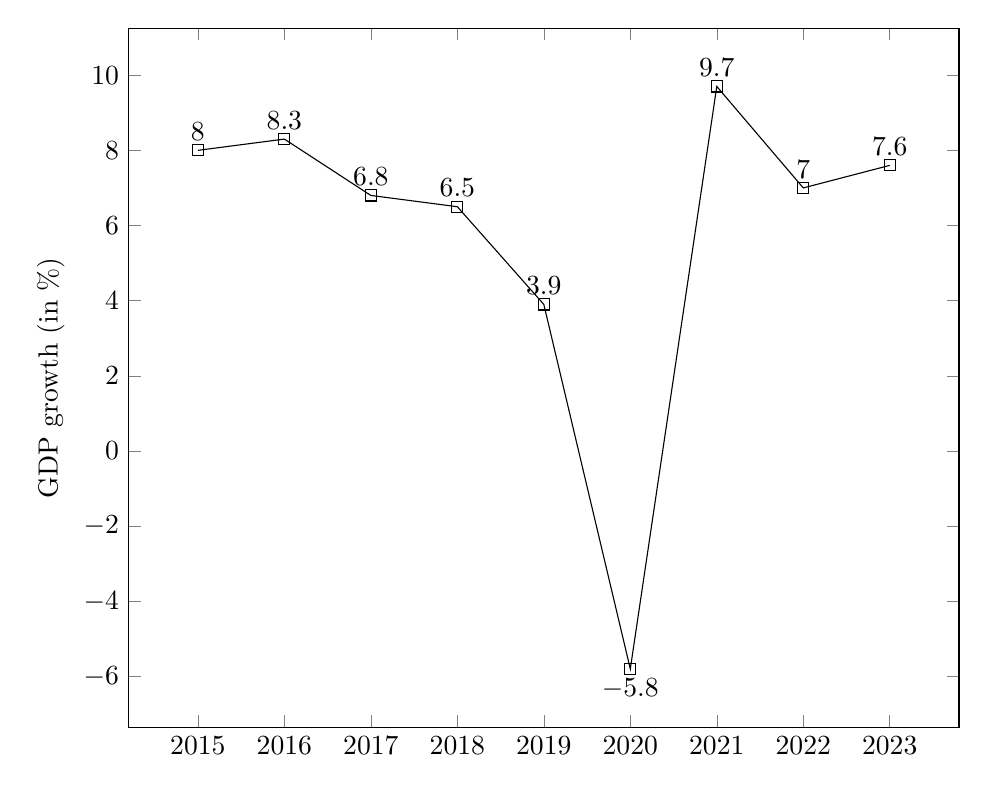
\begin{tikzpicture}
    \begin{axis}[
    xlabel={},
    width=\textwidth,
    mark=square,
    ylabel={GDP growth (in \%)},
    % remove comma in xticklabels
    xticklabel style={/pgf/number format/set thousands separator={}},
    xtick distance=1,
    nodes near coords
    ]
    \addplot[color=black, x={Year}, y={GDP growth (in \%)}] table {
    2015 8
    2016 8.3
    2017 6.8
    2018 6.5
    2019 3.9
    2020 -5.8
    2021 9.7
    2022 7
    2023 7.6
    };
    \end{axis}
    \end{tikzpicture}
\end{center}
\begin{floatsource}
Source: World Bank
\end{floatsource}
\end{figure}

\section{Section Name}
\lipsum
\section{Conclusion}
\lipsum
\end{document}